\section{Module operation}\label{sec:operation}
This section provides a guide to configuring and operating the low-frequency components, focusing on initialization, operating modes, and control logic.

\subsection{Initialization sequence}

\begin{itemize}[nosep]
    \item After a system reset (active low), the SPI Slave Interface enters an Idle state, setting spi\_busy to inactive (high).
    \item Configuration inputs (cpol, cpha, bit\_order) must be set before any transaction begins to define clock polarity, phase, and data order.
    \item The system awaits slave select (i\_ss) activation (active low) from the external SPI Master to initiate a transaction.
\end{itemize}


\subsection{Operating Modes and Use-Cases}

\begin{itemize}[nosep]
    \item \textbf{Write Mode (Data Reception)}:
    \begin{itemize}[nosep]
        \item \textbf{Trigger}: Operation bit received as 0 via i\_mosi.
        \item \textbf{Steps}:
        \begin{enumerate}[nosep]
            \item SPI Slave Interface sets spi\_busy to active (low) and forwards serial data to Deserializer and CRC Block.
            \item Deserializer converts data to parallel format (data\_block[15:0]) and then outputs to synchronization register and comparator (data\_block[15:8] for CRC).
            \item CRC Block generates crc\_code[7:0] for comparison at the comparator.
            \item If valid, data is forwarded to sync device; if invalid, error feedback is generated.
            \item Supports burst transactions by looping reception while i\_ss remains active.
        \end{enumerate}
    \end{itemize}
    \item \textbf{Read Mode (Data Transmission)}:
    \begin{itemize}[nosep]
        \item \textbf{Trigger}: Operation bit received as 1 via i\_mosi.
        \item \textbf{Steps}:
        \begin{enumerate}[nosep]
            \item SPI Slave Interface sets spi\_busy to active (low) and signals to fetch parallel data.
            \item Parallel data (parallel\_data[7:0]) from async FIFO or other source is sent to Serializer, while CRC Block generates crc\_code[7:0].
            \item Serializer converts data and CRC to serial format (o\_miso) for transmission via o\_miso.
            \item Supports burst transactions by fetching additional data while i\_ss remains active.
        \end{enumerate}
    \end{itemize}
    \item \textbf{Use-Case Notes}: Both modes adhere to the data format (4-bit operation field, 12-bit address, 16-bit data, 8-bit CRC) and operate under sck timing up to 1 MHz.
\end{itemize}

\subsection{Interrupts and status flags}

\begin{itemize}
    \item \textbf{spi\_busy}: Active low signal indicating an ongoing SPI transaction, set during operation detection, reception, validation, and transmission states. Used by internal system components to monitor transaction status.
    \item \textbf{Error Feedback}: Generated by the comparator during write mode if CRC validation fails (data\_block[15:8] does not match crc\_code[7:0]), signaling an integrity issue with received data. Specific interrupt mechanisms will be defined in system-level integration.
\end{itemize}

\subsection{Finite state machine (FSM) design}

The control logic is managed by an FSM within the SPI Slave Interface, detailed as follows:

\begin{itemize}[nosep]
    \item \textbf{State Definitions for Write Flow}:
    \begin{itemize}[nosep]
        \item \textbf{Idle State}: Wait for transaction initiation (ss active low), spi\_busy inactive.
        \item \textbf{Config State}: Read configuration settings (cpol, cpha, bit\_order).
        {\sloppy
        \item \textbf{Operation Detect State}: Determine operation type (0 for write), set spi\_busy active.
        \par}
        \item \textbf{Receive State}: Forward i\_mosi data to Deserializer and CRC Block, track bit count for data segments.
        \item \textbf{Validate State}: Compare CRC for integrity, forward valid data or generate error feedback.
    \end{itemize}
    \item \textbf{State Definitions for Read Flow}:
    \begin{itemize}
        \item \textbf{Idle, Config, Operation Detect States}: Shared with write flow, transition to Transmit on operation bit 1 (read).
        \item \textbf{Transmit State}: Fetch parallel data, serialize with CRC, transmit the data via o\_miso, support burst if i\_ss active.
    \end{itemize}
    \item \textbf{FSM Diagram}:
    \begin{figure}[!htb]
        \centering
        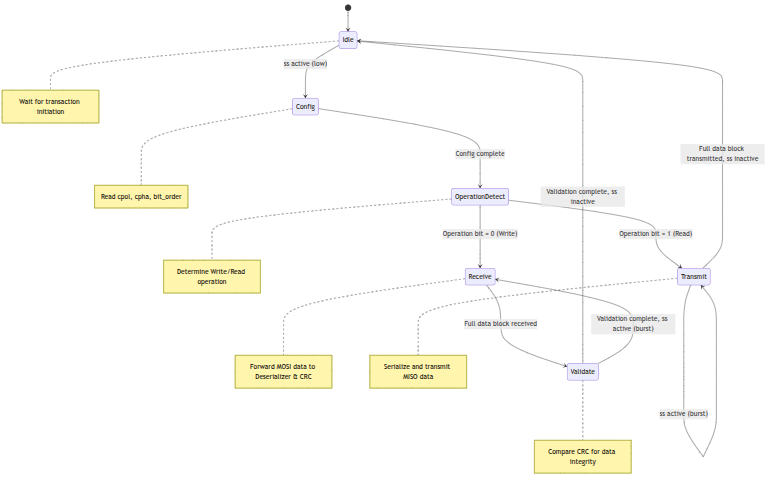
\includegraphics[width=1\linewidth]{figures/fsm-design.png}
        \caption{FSM design}
        \label{fig:fsm-design}
    \end{figure}
\end{itemize}
